% ==============================================================================
% PAGE 28: 10) BATTERY(6V,6AMP) (Numbered Page 20)
% ==============================================================================
\subsubsection*{10) BATERY(6V,6AMP)}

\begin{center}
  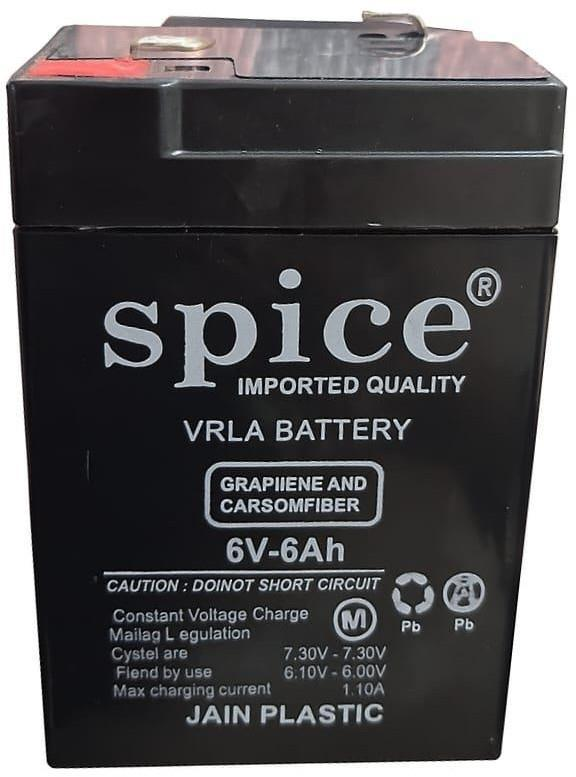
\includegraphics[width=55mm]{figures/fig12_battery.jpg}
\end{center}

\noindent
\begin{spacing}{1.2}
{\fontsize{10.2}{14.5}\selectfont
The system uses a Spice VRLA Battery (6V, 6Ah) made with graphene and carbon fiber technology. It is a sealed lead-acid, maintenance-free battery that provides stable DC power for operating the motor and sensors.\\[3mm]
\textbf{Main Specifications:}
\begin{itemize}[leftmargin=8mm, itemsep=1.5mm, label=\textbullet]
  \item \textbf{Type:} VRLA (Valve Regulated Lead Acid) Battery
  \item \textbf{Rated Voltage:} 6V
  \item \textbf{Capacity:} 6Ah
  \item \textbf{Charging Voltage:} 7.2V -- 7.5V (Cycle use)
  \item \textbf{Standby Voltage:} 6.78V -- 6.90V
  \item \textbf{Maximum Charging Current:} 1.35A
  \item \textbf{Features:} Maintenance-free, long service life, and safe sealed design
\end{itemize}
\vspace{2mm}
This battery ensures reliable power supply for small DC motors and electronic sensor circuits in the project.
}
\end{spacing}
\clearpage
